\documentclass[aspectratio=169]{beamer}
\usetheme{Madrid}
\usecolortheme{default}

% Packages
\usepackage{graphicx}
\usepackage{tikz}
\usepackage{array}
\usepackage{booktabs}
\usetikzlibrary{shapes.geometric, arrows, positioning}

% Color scheme
\definecolor{primaryblue}{RGB}{0,102,204}
\definecolor{secondarygreen}{RGB}{0,153,76}
\setbeamercolor{structure}{fg=primaryblue}
\setbeamercolor{frametitle}{bg=primaryblue,fg=white}

% Title Information
\title{SanitiSense AI}
\subtitle{Bridging Citizens and Civic Systems Through Intelligent Sanitation Reporting}
\author{Team Name: SanitiSense AI}
\date{\today}

\begin{document}

% Title Slide
\begin{frame}
\titlepage
\end{frame}

%------------------------------------------------------------
% Slide 1: Team Information
%------------------------------------------------------------
\begin{frame}{Team Information}

\begin{block}{Team Name}
\Large{\textbf{SanitiSense AI}}
\end{block}

\vspace{0.5cm}

\begin{block}{Problem Statement}
Residents in underserved communities fail to get sanitation hazards (overflowing drains, garbage accumulation) resolved because municipal systems prioritize formal, written, and categorized grievances, ignoring unstructured photo- and voice-based reports.
\end{block}

\vspace{0.5cm}

\begin{block}{Team Leader Name}
\textbf{<Your Name>}
\end{block}

\end{frame}

%------------------------------------------------------------
% Slide 2: Brief About the Idea
%------------------------------------------------------------
\begin{frame}{Brief About the Idea}

\begin{itemize}
    \item \textbf{SanitiSense AI} is an AI-powered system that enables low-literacy citizens to report sanitation hazards using a photo and an optional voice note
    \vspace{0.3cm}
    \item The system \textbf{verifies} the issue using computer vision
    \vspace{0.3cm}
    \item \textbf{Extracts contextual urgency} from voice input
    \vspace{0.3cm}
    \item \textbf{Converts} informal citizen reports into structured, evidence-backed civic tickets that authorities can act upon
\end{itemize}

\vspace{0.5cm}

\begin{alertblock}{Core Philosophy}
Instead of creating another complaint portal, the solution acts as an \textbf{intelligent translation layer} between citizen reality and municipal systems.
\end{alertblock}

\end{frame}

%------------------------------------------------------------
% Slide 3: How Is This Different From Existing Solutions? (USP)
%------------------------------------------------------------
\begin{frame}{How Is This Different From Existing Solutions?}

\begin{columns}[T]
\begin{column}{0.48\textwidth}
\textbf{\color{red}Existing Systems:}
\begin{itemize}
    \item Require written, form-based complaints
    \item Reject or ignore unstructured WhatsApp or verbal reports
    \item Lack prioritization and aggregation of citizen complaints
\end{itemize}
\end{column}

\begin{column}{0.48\textwidth}
\textbf{\color{secondarygreen}Our Differentiation (USP):}
\begin{itemize}
    \item Image-first reporting ensures evidence-based verification
    \item AI filters spam and invalid submissions automatically
    \item Converts vernacular, unstructured inputs into structured civic data
    \item Aggregates repeated issues to expose ignored sanitation hotspots
\end{itemize}
\end{column}
\end{columns}

\vspace{0.5cm}

\begin{center}
\Large{\textbf{\color{primaryblue}``We don't help citizens complain — we help systems understand.''}}
\end{center}

\end{frame}

%------------------------------------------------------------
% Slide 4: How Does the Solution Solve the Problem?
%------------------------------------------------------------
\begin{frame}{How Does the Solution Solve the Problem?}

\begin{enumerate}
    \item Citizens submit a \textbf{photo} of a sanitation issue (mandatory)
    \vspace{0.3cm}
    \item \textbf{Optional voice note} provides context such as duration, smell, or obstruction
    \vspace{0.3cm}
    \item \textbf{AI validates} whether the image represents a real sanitation hazard
    \vspace{0.3cm}
    \item The system \textbf{classifies issue type} and estimates severity
    \vspace{0.3cm}
    \item \textbf{Structured and prioritized} sanitation tickets are generated automatically
    \vspace{0.3cm}
    \item \textbf{Repeated complaints} are clustered to identify high-risk zones
\end{enumerate}

\vspace{0.3cm}

\begin{block}{Impact}
This removes literacy, language, and documentation barriers while enabling accountability.
\end{block}

\end{frame}

%------------------------------------------------------------
% Slide 5: Features Offered by the Solution
%------------------------------------------------------------
\begin{frame}{Features Offered by the Solution}

\begin{columns}[T]
\begin{column}{0.48\textwidth}
\textbf{Image Processing:}
\begin{itemize}
    \item Image-based sanitation issue detection and validation
    \item Automatic spam and irrelevant image rejection
    \item Severity estimation using visual cues (scale, spread, obstruction)
\end{itemize}
\end{column}

\begin{column}{0.48\textwidth}
\textbf{Voice \& Analytics:}
\begin{itemize}
    \item Voice-based context capture in local languages
    \item NLP-based extraction of urgency indicators
    \item Clustering of repeated complaints into sanitation hotspots
    \item Evidence-backed dashboard for authorities or NGOs
\end{itemize}
\end{column}
\end{columns}

\end{frame}

%------------------------------------------------------------
% Slide 6: Process Flow
%------------------------------------------------------------
\begin{frame}{Process Flow}

\begin{center}
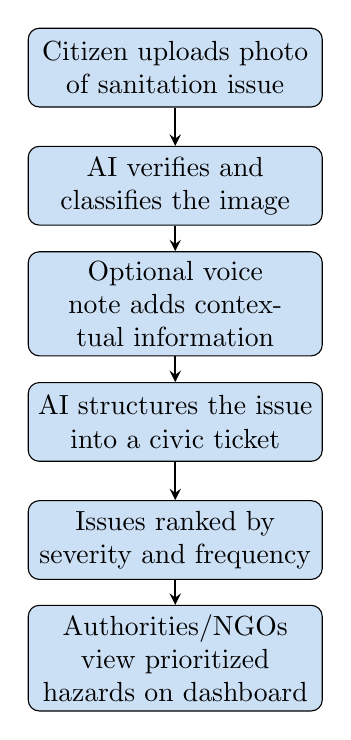
\begin{tikzpicture}[node distance=1.5cm, auto,
    box/.style={rectangle, draw, fill=primaryblue!20, text width=3.5cm, align=center, minimum height=1cm, rounded corners},
    arrow/.style={->, >=stealth, thick}]
    
    \node[box] (upload) {Citizen uploads photo of sanitation issue};
    \node[box, below of=upload] (verify) {AI verifies and classifies the image};
    \node[box, below of=verify] (voice) {Optional voice note adds contextual information};
    \node[box, below of=voice] (structure) {AI structures the issue into a civic ticket};
    \node[box, below of=structure] (rank) {Issues ranked by severity and frequency};
    \node[box, below of=rank] (dashboard) {Authorities/NGOs view prioritized hazards on dashboard};
    
    \draw[arrow] (upload) -- (verify);
    \draw[arrow] (verify) -- (voice);
    \draw[arrow] (voice) -- (structure);
    \draw[arrow] (structure) -- (rank);
    \draw[arrow] (rank) -- (dashboard);
\end{tikzpicture}
\end{center}

\end{frame}

%------------------------------------------------------------
% Slide 7: Wireframes / Mock Diagrams
%------------------------------------------------------------
\begin{frame}{Wireframes / Mock Diagrams}

\begin{columns}[T]
\begin{column}{0.48\textwidth}
\textbf{Citizen Interface:}
\begin{center}
\begin{tikzpicture}
    \draw[thick] (0,0) rectangle (3,5);
    \node at (1.5,4.5) {\textbf{SanitiSense AI}};
    
    \draw[fill=gray!30] (0.3,2.5) rectangle (2.7,4);
    \node at (1.5,3.5) {📷};
    \node at (1.5,3) {\small Upload Photo};
    
    \draw[fill=gray!20] (0.3,1.5) rectangle (2.7,2.3);
    \node at (1.5,1.9) {🎤 Record Voice Note};
    
    \draw[fill=primaryblue!50] (0.5,0.3) rectangle (2.5,1);
    \node at (1.5,0.65) {\textcolor{white}{\textbf{Submit}}};
\end{tikzpicture}
\end{center}
\end{column}

\begin{column}{0.48\textwidth}
\textbf{Dashboard Interface:}
\begin{center}
\begin{tikzpicture}[scale=0.85]
    \draw[thick] (0,0) rectangle (4,5);
    \node at (2,4.7) {\textbf{Sanitation Dashboard}};
    
    \draw[fill=red!30] (0.2,3.8) rectangle (3.8,4.5);
    \node[text width=3cm, align=center] at (2,4.15) {\tiny High Severity Issues};
    
    \draw[fill=orange!30] (0.2,3) rectangle (3.8,3.7);
    \node[text width=3cm, align=center] at (2,3.35) {\tiny Medium Severity Issues};
    
    \draw[fill=yellow!30] (0.2,2.2) rectangle (3.8,2.9);
    \node[text width=3cm, align=center] at (2,2.55) {\tiny Low Severity Issues};
    
    \node[text width=3.5cm, align=center] at (2,1.5) {\tiny 📍 Hotspot Areas Highlighted};
    
    \node[text width=3.5cm, align=center] at (2,0.7) {\tiny ✓ Visual Evidence Attached};
\end{tikzpicture}
\end{center}
\end{column}
\end{columns}

\end{frame}

%------------------------------------------------------------
% Slide 8: Architecture Diagram
%------------------------------------------------------------
\begin{frame}{Architecture Diagram of the Proposed Solution}

\begin{center}
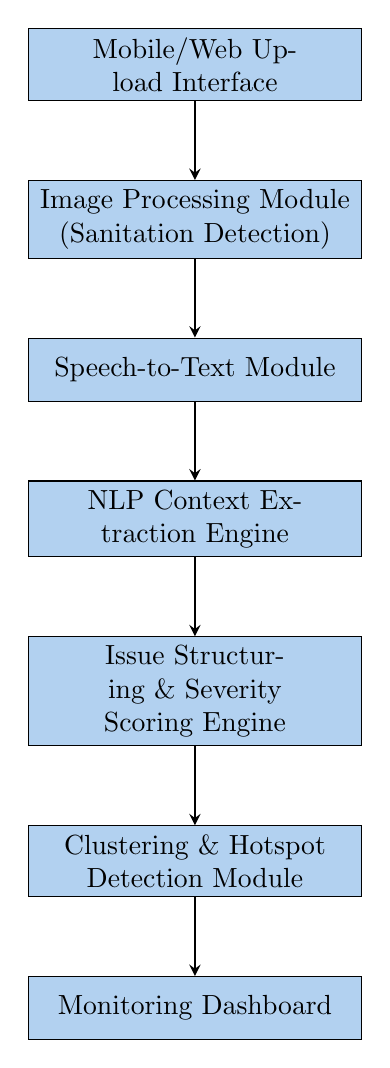
\begin{tikzpicture}[node distance=1cm, auto,
    layer/.style={rectangle, draw, fill=primaryblue!30, text width=4cm, align=center, minimum height=0.8cm},
    arrow/.style={->, >=stealth, thick}]
    
    \node[layer] (interface) {Mobile/Web Upload Interface};
    \node[layer, below=of interface] (image) {Image Processing Module\\(Sanitation Detection)};
    \node[layer, below=of image] (speech) {Speech-to-Text Module};
    \node[layer, below=of speech] (nlp) {NLP Context Extraction Engine};
    \node[layer, below=of nlp] (scoring) {Issue Structuring \& Severity\\Scoring Engine};
    \node[layer, below=of scoring] (clustering) {Clustering \& Hotspot\\Detection Module};
    \node[layer, below=of clustering] (dashboard) {Monitoring Dashboard};
    
    \draw[arrow] (interface) -- (image);
    \draw[arrow] (image) -- (speech);
    \draw[arrow] (speech) -- (nlp);
    \draw[arrow] (nlp) -- (scoring);
    \draw[arrow] (scoring) -- (clustering);
    \draw[arrow] (clustering) -- (dashboard);
\end{tikzpicture}
\end{center}

\end{frame}

%------------------------------------------------------------
% Slide 9: Technologies to Be Used
%------------------------------------------------------------
\begin{frame}{Technologies to Be Used}

\begin{itemize}
    \item \textbf{Computer Vision} for sanitation image classification
    \vspace{0.4cm}
    \item \textbf{Speech-to-Text} for local language voice input
    \vspace{0.4cm}
    \item \textbf{Natural Language Processing} for context extraction
    \vspace{0.4cm}
    \item \textbf{Rule-based + lightweight ML models} for severity scoring
    \vspace{0.4cm}
    \item \textbf{Spatial clustering} for hotspot detection
    \vspace{0.4cm}
    \item \textbf{Cloud-based backend} for scalability
\end{itemize}

\end{frame}

%------------------------------------------------------------
% Slide 10: Estimated Implementation Cost
%------------------------------------------------------------
\begin{frame}{Estimated Implementation Cost}

\begin{block}{Cost-Effective Approach}
\begin{itemize}
    \item Uses \textbf{lightweight inference models} suitable for low-cost cloud deployment
    \vspace{0.3cm}
    \item \textbf{No continuous human moderation} required
    \vspace{0.3cm}
    \item Suitable for \textbf{NGO pilots or ward-level rollouts}
    \vspace{0.3cm}
    \item \textbf{Pay-per-use or subscription-based} operational cost
\end{itemize}
\end{block}

\vspace{0.5cm}

\begin{center}
\textit{Scalable from pilot to city-wide deployment}
\end{center}

\end{frame}

%------------------------------------------------------------
% Slide 11: Expected Impact
%------------------------------------------------------------
\begin{frame}{Expected Impact}

\begin{block}{Key Outcomes}
\begin{itemize}
    \item \textbf{Increased acknowledgment} of valid sanitation complaints
    \vspace{0.3cm}
    \item \textbf{Faster response} to high-severity sanitation hazards
    \vspace{0.3cm}
    \item \textbf{Reduced repeat complaints} from the same areas
    \vspace{0.3cm}
    \item \textbf{Improved accountability} through evidence-backed reporting
\end{itemize}
\end{block}

\vspace{0.5cm}

\begin{center}
\Large{\textbf{\color{secondarygreen}Building Trust Between Citizens and Civic Systems}}
\end{center}

\end{frame}

%------------------------------------------------------------
% Thank You Slide
%------------------------------------------------------------
\begin{frame}
\begin{center}
\Huge{\textbf{Thank You}}

\vspace{1cm}

\Large{Questions?}

\vspace{1cm}

\normalsize{\textbf{Team: SanitiSense AI}}
\end{center}
\end{frame}

\end{document}
